\documentclass{standalone}
\usepackage{tikz}
\usepackage{ctex,siunitx}
\setCJKmainfont{Noto Serif CJK SC}
\usepackage{tkz-euclide}
\usepackage{amsmath}
\usetikzlibrary{patterns, calc,3d}
\usetikzlibrary {decorations.pathmorphing,decorations.pathreplacing,decorations.shapes}
\begin{document}
\small
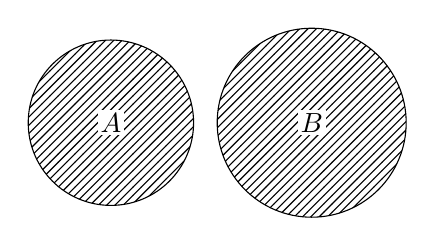
\begin{tikzpicture}[>=latex,scale=1.5,inner sep=1pt]
  \draw[pattern=north east lines](-0.8,0)circle(0.7)node[fill=white]{$A$};
  \draw[pattern=north east lines](0.9,0)circle(0.8)node[fill=white]{$B$};
\end{tikzpicture}
\end{document}